\section{Pendahuluan}
\subsection{Latar Belakang}
Komunikasi dan transfer data merupakan aspek penting dalam sistem komputer modern. Komunikasi dan transfer data antar perangkat sejatinya dapat dilakukan dengan metode copy-paste konvensional dengan menyalin data yang akan dikirim ke external storage device dari komputer pengirim lalu membawa dan menghubungkan external storage device tersebut ke komputer penerima, yang kemudian akan menyalin data dari pengirim yang telah disimpan pada storage device. Metode sangat mudah dilakukan, namun seiring dengan berkembangnya zaman, kebutuhan data yang akan ditransfer semakin banyak dan besar serta jarak fisik antara komputer pengirim dan komputer penerima juga semakin jauh, sehingga metode transfer data menggunakan external device seperti USB Drive atau disket menjadi tidak efisien karena harus memindahkan external device secara fisik dari satu tempat ke tempat lain. Oleh karena itu, diperlukan sebuah cara untuk memindahkan data dari satu komputer ke komputer lain secara cepat dan tanpa harus berpindah tempat secara fisik. 

Permasalahan ini dapat diselesaikan dengan menghubungkan komputer-komputer yang akan berkomunikasi ke dalam sebuah jaringan. Dengan membuat sebuah jaringan, maka komputer-komputer dan perangkat-perangkat yang berada dalam jaringan tersebut dapat berkomunikasi dan mengirim data satu sama lain tanpa harus memindahkan data-data tersebut secara manual menggunakan external device. Jaringan komputer yang paling dasar adalah sebuah jaringan LAN yang dihubungkan dengan kabel UTP dan alamat-alamat perangkat yang dirouting menggunakan protokol IPv4. Untuk dapat memahami bagaimana jaringan komputer bekerja, tentu saja diperlukan pemahaman akan kedua hal tersebut. Maka dari itu dilakukan praktikum crimping dan routing IPv4 untuk lebih memahami bagaimana kabel UTP dapat menghubungkan komputer dalam sebuah jaringan dan bagaimana protokol IPv4 membuat komputer dapat berkomunikasi satu sama lain.

\subsection{Dasar Teori}
Kabel UTP (Unshielded Twisted Pair) merupakan kabel yang digunakan sebagai media fisik bagi perangkat dalam sebuah jaringan untuk berkomunikasi satu sama lain. Kabel ini pada umumnya digunakan dalam lingkup jaringan skala kecil seperti LAN (Local Area Network). Dalam sebuah kabel UTP, terdapat 8 kabel dengan kode warna berbeda. 8 kabel ini memiliki fungsi berbeda-beda sesuai dengan kode warnanya. Kabel berwarna putih-oranye berfungsi sebagai sisi positif penghantar data, kabel berwarna oranye berfungsi sebagai sisi negatif penghantar data, kabel berwarna putih-hijau berfungsi sebagai sisi positif penerima data, kabel berwarna hijau berfungsi sebagai sisi negatif penerima data, kabel berwarna putih-biru berfungsi sebagai sisi positif penghantar paket suara, kabel berwarna biru berfungsi sebagai sisi negatif penghantar paket suara, kabel berwarna putih-coklat berfungsi sebagai sisi positif penghantar tengangan DC, dan kabel berwarna coklat berfungsi sebagai sisi negatif penghantar tengangan DC. Dalam jaringan komputer, kabel yang digunakan hanyalah kabel putih-oranye, oranye, putih-hijau, dan hijau. Kabel putih-biru dan biru digunakan dalam telepon, kabel putih-coklat dan coklat digunakan dalam PoE (Power over Ethernet). Untuk dapat terhubung ke komputer atau router, kabel UTP harus dihubungkan menggunakan konektor RJ45. Proses menata kabel UTP ke konektor RJ45 disebut dengan proses crimping. Tatanan konfigurasi warna kabel UTP saat crimping dapat dibedakan menjadi dua, yaitu T568A dan T568B. T568A memiliki urutan warna (dari kiri ke kanan) putih-hijau, hijau, putih-oranye, biru, putih-biru, oranye, putih-coklat, dan coklat. T668B memiliki urutan warna (dari kiri ke kanan) putih-oranye, oranye, putih-hijau, biru, putih-biru, hijau, putih-coklat, dan coklat. Berdasarkan pemasangannya, konfigurasi kabel UTP dapat dibagi menjadi straight-through dan crossover. Straight-through digunakan untuk menghubungkan perangkat dengan tipe yang berbeda, yaitu DTE (Data Terminal Equipment, contohnya komputer, mikrokomputer, printer) ke DCE (Data Circuit-terminating Equipment, contohnya router dan switch). Pada konfigurasi straight-through, kedua ujung kabel memiliki konfigurasi warna yang sama, misalnya bila pada satu ujung menggunakan T568B maka ujung lainnya juga harus mengguunakan T568B. Crossover digunakan untuk mengubungkan perangkat dengan tipe yang sama, yaitu DTE ke DTE atau DCE ke DCE. Pada konfigurasi crossover, kedua ujung kabel harus menggunakan konfigurasi warna yang berbeda, misal pada satu ujung menggunakan konfigurasi T568A maka ujung lainnya harus menggunakan T568B. 

IPv4 merupakan protokol internet (IP) versi keempat sekaligus versi yang paling umum digunakan saat ini. IPv4 terdiri atas nilai 32 bit yang dipisahkan menjadi 4 bagian yang disebut oktet, dengan satu oktet merupakan angka desimal yang dipisahkan oleh titik dan terdiri atas 8 bit. Alamat IPv4 menentukan identitas logis perangkat pada jaringan, sehingga selama komunikasi antar perangkat terjadi data dapat dikirimkan ke tempat yang jelas dan sepsifik berdasarkan alamat IP. Alamat IP pada IPv4 dibagi menjadi 3 bagian, yaitu network part, host part, dan subnet part. Network part merupakan bagian yang menunjukkan jaringan utama dari host, sehingga semua host yang tergabung dalam satu jaringan yang sama memiliki nilai network part yang identik. Host part merupakan bagian yang menunjukkan identitas unik host pada jaringan, sehingga setiap perangkat/host pada satu jaringan yang sama memiliki nilai host part yang berbeda-beda. Subnet part merupakan bagian yang menunjukkan subnet tempat host berada. Dalam format penulisan alamat berkelas (classful), network part dan host part ditentukan oleh kelas alamat. Network part untuk kelas A adalah oktet pertama, untuk kelas B adalah oktet pertama hingga kedua, dan untuk kelas C adalah oktet pertama hingga ketiga. Sisanya adalah host part dan subnet part bila dalam jaringan terdapat subnet. Dalam format penulisan CIDR, network part ditentukan oleh nilai notasi CIDR. Misal pada alamat IP dengan format CIDR 192.168.0.0/24, notasi /24 menandakan bahwa 24 bit digunakan sebagai network part dan sisanya (8 bit) digunakan sebagai host part.

%===========================================================%
\section{Tugas Pendahuluan}
\begin{enumerate}
	\item Misalkan IP address jaringan internal perusahaan adalah 192.168.0.xxx, maka rentang IP dan prefix untuk tiap departemen adalah:
	\\
	Departemen produksi: Rentang: 192.168.0.128 - 192.168.0.191, prefix: /26
	\\
	Departemen administrasi: Rentang: 192.168.0.192 - 192.168.0.223, prefix: /27
	\\
	Departemen keuangan: Rentang: 192.168.0.224 - 192.168.0.239, prefix: /28
	\\
	Departemen R\&D: Rentang: 192.168.0.0 - 192.168.0.127, prefix: /25
	\\
	Total subnet yang diperlukan adalah 4 subnet, dengan 1 subnet untuk masing-masing departemen. IP network untuk masing-masing subnet adalah:
	\\
	Departemen produksi: 192.168.0.128/26
	\\
	Departemen administrasi: 192.168.0.192/27
	\\
	Departemen keuangan: 192.168.0.224/28
	\\
	Departemen R\&D: 192.168.0.0/25
	\item Berikut adalah topologi dari jaringan perusahaan. Satu PC mewakili 10 perangkat pada masing-masing departemen
	\begin{figure}[H]
		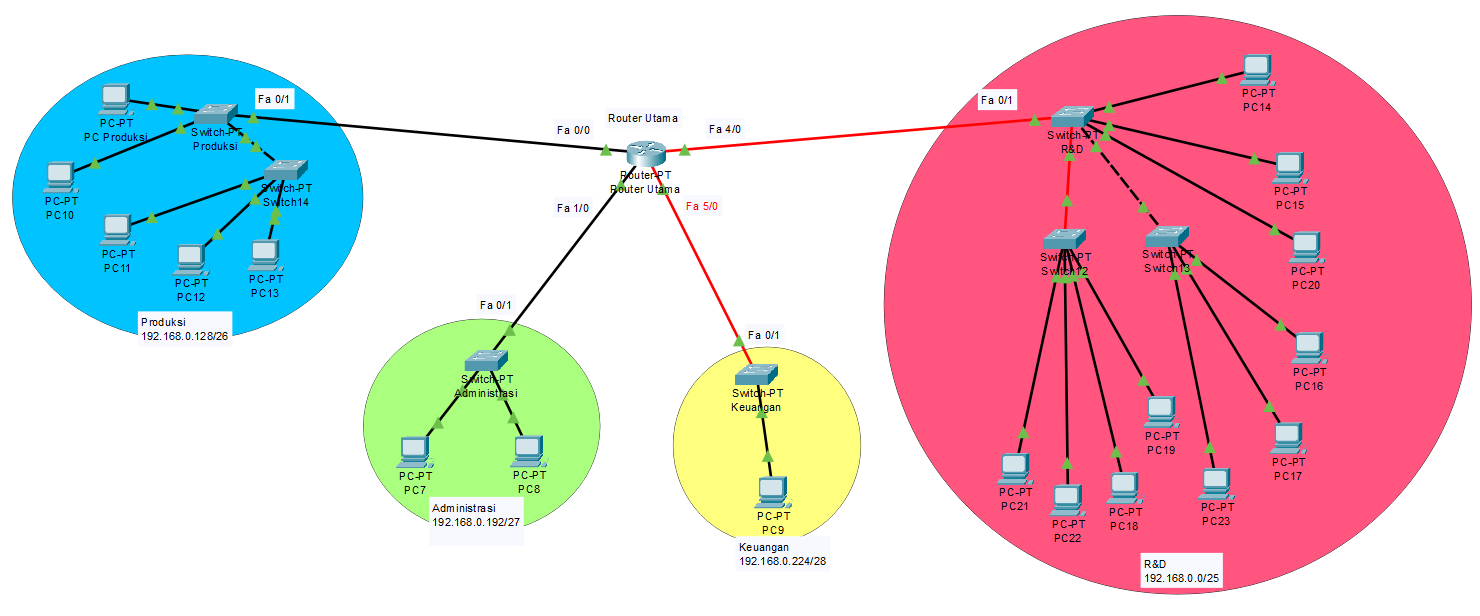
\includegraphics[scale=0.45]{P1/img/topologi-tupen-r.png}
	\end{figure}
	\item Tabel routing subnet departemen produksi:\\
	\begin{tabular}{| c | c | c | c |}
		\hline
		Destination & Netmask & Gateway & Interface\\
		\hline
		192.168.0.0 & 255.255.255.128 & 192.168.0.129 & Fa 4/0 \\
		\hline
		192.168.0.128 & 255.255.255.192 & on-link & Fa 0/0\\
		\hline
		192.168.0.192 & 255.255.255.224 & 192.168.0.129 & Fa 1/0\\
		\hline
		192.168.0.224 & 255.255.255.240 & 192.168.0.129 & Fa 5/0\\
		\hline
	\end{tabular}\\\\
	Tabel routing subnet departemen administrasi:\\
	\begin{tabular}{| c | c | c | c |}
		\hline
		Destination & Netmask & Gateway & Interface\\
		\hline
		192.168.0.0 & 255.255.255.128 & 192.168.0.193 & Fa 4/0 \\
		\hline
		192.168.0.128 & 255.255.255.192 & 192.168.0.193 & Fa 0/0\\
		\hline
		192.168.0.192 & 255.255.255.224 & on-link & Fa 1/0\\
		\hline
		192.168.0.224 & 255.255.255.240 & 192.168.0.193 & Fa 5/0\\
		\hline
	\end{tabular}\\\\
	Tabel routing subnet departemen keuangan:\\
	\begin{tabular}{| c | c | c | c |}
		\hline
		Destination & Netmask & Gateway & Interface\\
		\hline
		192.168.0.0 & 255.255.255.128 & 192.168.0.225 & Fa 4/0 \\
		\hline
		192.168.0.128 & 255.255.255.192 & 192.168.0.225 & Fa 0/0\\
		\hline
		192.168.0.192 & 255.255.255.224 & 192.168.0.225 & Fa 1/0\\
		\hline
		192.168.0.224 & 255.255.255.240 & on-link & Fa 5/0\\
		\hline
	\end{tabular}\\\\
	Tabel routing subnet departemen R\&D:\\
	\begin{tabular}{| c | c | c | c |}
		\hline
		Destination & Netmask & Gateway & Interface\\
		\hline
		192.168.0.0 & 255.255.255.128 & on-link & Fa 4/0 \\
		\hline
		192.168.0.128 & 255.255.255.192 & 192.168.0.1 & Fa 0/0\\
		\hline
		192.168.0.192 & 255.255.255.224 & 192.168.0.1 & Fa 1/0\\
		\hline
		192.168.0.224 & 255.255.255.240 & 192.168.0.1 & Fa 5/0\\
		\hline
	\end{tabular}\\\\
	
	\item Routing yang paling cocok adalah routing berbasis classless inter-domain routing (CIDR). Routing ini cocok karena penggunaan CIDR memungkinkan routing yang lebih efisien dan fleksibel. CIDR memungkinkan penggunaan alamat IP yang lebih efisien dan fleksibel karena penggunaan alamat IP bisa diesuaikan dengan jumlah host yang dimiliki perusahaan dengan menyesuaikan prefix alamat dengan jumlah host sehingga meminimalisir pemborosan alamat IP dan dapat disesuaikan atau diatur ulang apabila sewaktu-waktu jumlah host bertambah atau berkurang, berbeda dengan routing yang berbasis alamat IP classful yang jumlah hostnya ditentukan oleh kelas alamat sehingga kurang fleksibel.
\end{enumerate}